%%%%% Set up %%%%%

% Set document style and font size
\documentclass[12pt]{article}\usepackage[]{graphicx}\usepackage[]{color}
%% maxwidth is the original width if it is less than linewidth
%% otherwise use linewidth (to make sure the graphics do not exceed the margin)
\makeatletter
\def\maxwidth{ %
  \ifdim\Gin@nat@width>\linewidth
    \linewidth
  \else
    \Gin@nat@width
  \fi
}
\makeatother

\definecolor{fgcolor}{rgb}{0.345, 0.345, 0.345}
\newcommand{\hlnum}[1]{\textcolor[rgb]{0.686,0.059,0.569}{#1}}%
\newcommand{\hlstr}[1]{\textcolor[rgb]{0.192,0.494,0.8}{#1}}%
\newcommand{\hlcom}[1]{\textcolor[rgb]{0.678,0.584,0.686}{\textit{#1}}}%
\newcommand{\hlopt}[1]{\textcolor[rgb]{0,0,0}{#1}}%
\newcommand{\hlstd}[1]{\textcolor[rgb]{0.345,0.345,0.345}{#1}}%
\newcommand{\hlkwa}[1]{\textcolor[rgb]{0.161,0.373,0.58}{\textbf{#1}}}%
\newcommand{\hlkwb}[1]{\textcolor[rgb]{0.69,0.353,0.396}{#1}}%
\newcommand{\hlkwc}[1]{\textcolor[rgb]{0.333,0.667,0.333}{#1}}%
\newcommand{\hlkwd}[1]{\textcolor[rgb]{0.737,0.353,0.396}{\textbf{#1}}}%
\let\hlipl\hlkwb

\usepackage{framed}
\makeatletter
\newenvironment{kframe}{%
 \def\at@end@of@kframe{}%
 \ifinner\ifhmode%
  \def\at@end@of@kframe{\end{minipage}}%
  \begin{minipage}{\columnwidth}%
 \fi\fi%
 \def\FrameCommand##1{\hskip\@totalleftmargin \hskip-\fboxsep
 \colorbox{shadecolor}{##1}\hskip-\fboxsep
     % There is no \\@totalrightmargin, so:
     \hskip-\linewidth \hskip-\@totalleftmargin \hskip\columnwidth}%
 \MakeFramed {\advance\hsize-\width
   \@totalleftmargin\z@ \linewidth\hsize
   \@setminipage}}%
 {\par\unskip\endMakeFramed%
 \at@end@of@kframe}
\makeatother

\definecolor{shadecolor}{rgb}{.97, .97, .97}
\definecolor{messagecolor}{rgb}{0, 0, 0}
\definecolor{warningcolor}{rgb}{1, 0, 1}
\definecolor{errorcolor}{rgb}{1, 0, 0}
\newenvironment{knitrout}{}{} % an empty environment to be redefined in TeX

\usepackage{alltt}

% File path to resources (style file etc)
\newcommand{\locRepo}{csas-style}

% Style file for DFO Technical Reports
\usepackage{\locRepo/tech-report}

% header-includes from R markdown entry
\usepackage{pdflscape}

%%%%% Variables %%%%%

% New definitions: Title, year, report number, authors
% Protect lower case words (i.e., species names) in \Addlcwords{}, in "TechReport.sty"
\newcommand{\trTitle}{Estimation of fork length using cranial measurements of sablefish (\emph{Anoplopoma fimbria}) in British Columbia}
\newcommand{\trYear}{2022}
\newcommand{\trReportNum}{nnn}
% Optional
\newcommand{\trAuthFootA}{Email: \link{mailto:Kathryn.Temple@dfo-mpo.gc.ca}{\nolinkurl{Kathryn.Temple@dfo-mpo.gc.ca}} \textbar{} telephone: (250) 756-7366}
\newcommand{\trAuthsLong}{Kathryn x. Temple and Lisa C. Lacko and Kendra R. Holt and MGL person}
\newcommand{\trAuthsBack}{Kathryn x. Temple, L.C. Lacko and Holt K.R. and MGL person}

% New definition: Address
\newcommand{\trAddy}{Pacific Biological Station\\
Fisheries and Oceans Canada, 3190 Hammond Bay Road\\
Nanaimo, British Columbia, V9T 6N7, Canada\\}

% Abstract
\newcommand{\trAbstract}{Routine biological sampling of whole round sablefish from commercial fishing operations in British Columbia began the early 1990's. Historically, specimens have been obtained through the voluntary catch sampling and tag recovery programs. To increase the number of samples, we investigated the potential for obtaining sex and length information using heads, rather than the entire fish. In 2016, 438 sablefish (240-1080 mm) were sampled at sea and six different fish head measurements were collected. Genetic samples (137) were obtained to develop methods of DNA-based sex identification. A pilot study occurred in 2017 with 360 head-only samples collected and sexed by a commercial vessel, followed by scientific sampling on shore. Regression analysis results reveal that all six cranial dimensions can be used to accurately predict length. However, interorbital distance was not only a good predictor of length, but samplers ranked it the most efficient to measure and easily repeatable. Genomic DNA were successfully processed for 130 of the 137 samples. Fisher sex determination was accurate xx\% of the time. Given the results, the 2018 sampling collection program was modified so that returns of whole round sablefish were replaced by head-only samples with knife cuts on the operculum to indicate sex.}

% Resume (i.e., French abstract)
\newcommand{\trResume}{}

\newcommand{\trISBN}{}

\DeclareGraphicsExtensions{.png,.pdf}
%%%%% Start %%%%%

% Start the document
\IfFileExists{upquote.sty}{\usepackage{upquote}}{}

% commands and environments needed by pandoc snippets
% extracted from the output of `pandoc -s`
%% Make R markdown code chunks work
\usepackage{array}
\usepackage{amssymb,amsmath}
\usepackage{color}
\usepackage{fancyvrb}

% From default template:
\newcommand{\VerbBar}{|}
\newcommand{\VERB}{\Verb[commandchars=\\\{\}]}
\DefineVerbatimEnvironment{Highlighting}{Verbatim}{commandchars=\\\{\},formatcom=\color[rgb]{0.00,0.00,0.00}}
\usepackage{framed}
\definecolor{shadecolor}{RGB}{248,248,248}
\newenvironment{Shaded}{\begin{snugshade}}{\end{snugshade}}
\newcommand{\AlertTok}[1]{\textcolor[rgb]{0.94,0.16,0.16}{#1}}
\newcommand{\AnnotationTok}[1]{\textcolor[rgb]{0.56,0.35,0.01}{\textbf{\textit{#1}}}}
\newcommand{\AttributeTok}[1]{\textcolor[rgb]{0.77,0.63,0.00}{#1}}
\newcommand{\BaseNTok}[1]{\textcolor[rgb]{0.00,0.00,0.81}{#1}}
\newcommand{\BuiltInTok}[1]{#1}
\newcommand{\CharTok}[1]{\textcolor[rgb]{0.31,0.60,0.02}{#1}}
\newcommand{\CommentTok}[1]{\textcolor[rgb]{0.56,0.35,0.01}{\textbf{#1}}}
\newcommand{\CommentVarTok}[1]{\textcolor[rgb]{0.56,0.35,0.01}{\textbf{\textit{#1}}}}
\newcommand{\ConstantTok}[1]{\textcolor[rgb]{0.00,0.00,0.00}{#1}}
\newcommand{\ControlFlowTok}[1]{\textcolor[rgb]{0.13,0.29,0.53}{\textit{#1}}}
\newcommand{\DataTypeTok}[1]{\textcolor[rgb]{0.13,0.29,0.53}{#1}}
\newcommand{\DecValTok}[1]{\textcolor[rgb]{0.00,0.00,0.81}{#1}}
\newcommand{\DocumentationTok}[1]{\textcolor[rgb]{0.56,0.35,0.01}{\textbf{\textit{#1}}}}
\newcommand{\ErrorTok}[1]{\textcolor[rgb]{0.64,0.00,0.00}{\textit{#1}}}
\newcommand{\ExtensionTok}[1]{#1}
\newcommand{\FloatTok}[1]{\textcolor[rgb]{0.00,0.00,0.81}{#1}}
\newcommand{\FunctionTok}[1]{\textcolor[rgb]{0.00,0.00,0.00}{#1}}
\newcommand{\ImportTok}[1]{#1}
\newcommand{\InformationTok}[1]{\textcolor[rgb]{0.56,0.35,0.01}{\textbf{\textit{#1}}}}
\newcommand{\KeywordTok}[1]{\textcolor[rgb]{0.13,0.29,0.53}{\textit{#1}}}
\newcommand{\NormalTok}[1]{#1}
\newcommand{\OperatorTok}[1]{\textcolor[rgb]{0.81,0.36,0.00}{\textit{#1}}}
\newcommand{\OtherTok}[1]{\textcolor[rgb]{0.56,0.35,0.01}{#1}}
\newcommand{\PreprocessorTok}[1]{\textcolor[rgb]{0.56,0.35,0.01}{\textbf{#1}}}
\newcommand{\RegionMarkerTok}[1]{#1}
\newcommand{\SpecialCharTok}[1]{\textcolor[rgb]{0.00,0.00,0.00}{#1}}
\newcommand{\SpecialStringTok}[1]{\textcolor[rgb]{0.31,0.60,0.02}{#1}}
\newcommand{\StringTok}[1]{\textcolor[rgb]{0.31,0.60,0.02}{#1}}
\newcommand{\VariableTok}[1]{\textcolor[rgb]{0.00,0.00,0.00}{#1}}
\newcommand{\VerbatimStringTok}[1]{\textcolor[rgb]{0.31,0.60,0.02}{#1}}
\newcommand{\WarningTok}[1]{\textcolor[rgb]{0.56,0.35,0.01}{\textbf{\textit{#1}}}}
\begin{document}

%%%% Front matter %%%%%

% Add the first few pages
\frontmatter

%%%%% Drafts %%%%%

%\linenumbers  % Line numbers
%\onehalfspacing  % Extra space between lines
\renewcommand{\headrulewidth}{0.5pt}  % Header line
\renewcommand{\footrulewidth}{0.5pt}  % footer line
%\pagestyle{fancy}\fancyhead[c]{Draft: Do not cite or circulate}  % Header text

\newcommand{\lt}{\ensuremath <}
\newcommand{\gt}{\ensuremath >}

%Defines cslreferences environment
%Required by pandoc 2.8
%Copied from https://github.com/rstudio/rmarkdown/issues/1649
\newlength{\cslhangindent}
\setlength{\cslhangindent}{1.5em}
\newenvironment{cslreferences}%
  {}%
  {\par}

%%%%% Main document %%%%%
\hypertarget{introduction}{%
\section{Introduction}\label{introduction}}

Biological samples of British Columbia (BC) sablefish (\emph{Anoplopoma fimbria}) have been collected from a voluntary catch sampling program since 1995 (\protect\hyperlink{ref-Haist2001}{Haist and Wyeth 2001}) and processed by the Department of Fisheries and Oceans (DFO) port samplers and contracted service providers. In addition, whole tagged fish recovered in commercial fisheries (trap, trawl, hook and line) have been received at the point of landing via the dockside monitoring program (DMP) and sampled by Archipelago Marine Research (AMR) since the early 1990's. These data provide a fishery dependent source of age and size composition data for the two-sex structured operating model of the coastal Management Strategy Evaluation (MSE) (\protect\hyperlink{ref-Cox2019}{Cox et al. 2019}).

In recent years, a sablefish head only catch sampling and tagging program was developed in order to improve the number of returns from fishers, maintain the quality of the biological data and increase the range of fish sizes. Instead of returning the whole fish, commercial crew J-cut the fish as per commercial practice, view the gonads to determine sex, mark the sex with knife cuts on the operculum and store the head (and/or floy tag) for later sampling by DFO and AMR.

Previous research on other fish species has accurately estimated lengths from head dimensions (\protect\hyperlink{ref-Serafy1996}{Serafy et al. 1996}; \protect\hyperlink{ref-Park2007}{Park et al. 2007}), head and mandible lengths (\protect\hyperlink{ref-Isermann2005}{Isermann and Vandergoot 2005}), and head height to eye diameter ratio (\protect\hyperlink{ref-Richardson2015}{Richardson et al. 2015}). In this technical report we expand on previous research and describe the results of 1) the 2016 experimental study of cranial dimensions regressed against fork length; 2) the ease of each head measurement; 3) DNA sex detection methods; and 4) the compared consistency of the 2017 pilot study head measurements.

\hypertarget{methods}{%
\section{Methods}\label{methods}}

\hypertarget{experimental-study-2016}{%
\subsection{Experimental Study 2016}\label{experimental-study-2016}}

Sablefish were randomly selected for sampling during the 2016 biennial DFO Groundfish Synoptic Bottom Trawl surveys, following a length stratified protocol. A tally of 212 fish were sampled on the West Coast Vancouver Island survey (\protect\hyperlink{ref-Williams2018}{Williams et al. 2018}) and 219 fish were sampled on the West Coast Haida Gwaii survey (\protect\hyperlink{ref-Nottingham2018}{Nottingham et al. 2018}). In addition, seven small sablefish were collected during the 2016 salmon survey (Figure~\ref{fig:figure1}).

For each selected fish, fork length, round weight, sex and maturity were recorded at sea. The heads were removed, labelled and frozen. On shore, the cranial dimensions of upper jaw (L\textsubscript{UJ}), eye diameter (L\textsubscript{ED}), interorbital distance ( L\textsubscript{ID}), snout length (L\textsubscript{SL}), post orbital to preoperculum distance (L\textsubscript{PP}) and post orbital head length (L\textsubscript{PO}) were measured using Mitutoyo Absolute® 500-762-20 coolant proof digimatic calipers (Table~\ref{tab:table1}, Appendix~\ref{app:first-appendix}). Sagittal otoliths were collected for future ageing. Fork lengths (L\textsubscript{FL}) were estimated by a simple linear regression model, using the cranial measurements as a predictor variables.

At the time of sampling, each cranial dimension was evaluated by experienced samplers on a five point rating scale in terms of two distinct criteria: 1. ease of use and 2. repeatability. The ease of use metric focused on three key attributes of the measurement learn-ability (task understanding), efficiency (task-completion time) and degree of difficulty (task performance ease). The repeatability metric focused on ranking each measurement under repeated caliper placement, taking into consideration the soft and hard head tissues.

Operculum clips (DNA) were collected from the first 137 fish measured (79 male and 58 female) and forwarded to the Molecular Genetics Laboratory (MGL) for analysis and gender test development.

\hypertarget{molecular-genetics-laboratory-mgl-genetic-sex-determination}{%
\subsubsection{Molecular Genetics Laboratory (MGL) genetic sex-determination}\label{molecular-genetics-laboratory-mgl-genetic-sex-determination}}

DNA multiplex polymerase chain reactions (PCRs) were conducted using fluorescently labelled forward primers. X-insert and Y-insert specific primers developed by \protect\hyperlink{ref-Rondeau2013}{Rondeau et al.} (\protect\hyperlink{ref-Rondeau2013}{2013}) were used, but the X-insert forward and Y-nested reverse were redesigned to produce slightly smaller PCR products (Table~\ref{tab:table2}). Sex specific alleles were size fractionated in an ABI 3730 capillary DNA analyzer and were scored with ABI GeneMapper using an internal lane sizing standard.

\hypertarget{pilot-study-2017}{%
\subsection{Pilot study 2017}\label{pilot-study-2017}}

In 2017, a pilot study was conducted with the commercial sector returning sablefish head-only samples. A total of 360 heads were collected from J-cut sablefish on a limited-entry fishery trip to the Cobb and Eickelberg seamounts (Figure~\ref{fig:figure1}). Each operculum was marked by commercial fishers with either one knife cut (male) or two knife cuts (female) (Appendix~\ref{app:second-appendix}).

Scientific sampling occurred on shore, with the first 99 heads of the pilot study measured by three samplers for L\textsubscript{ID}, L\textsubscript{SL}, L\textsubscript{UJ} and L\textsubscript{PP}. Given that three highly experienced technicians were used to conduct the same measurements of the each head morphometric, the Index of Average Error (IAE) (Beamish 1981) was calculated to find the most consistent cranial measurement. It is defined as: \[
IAE=\frac{1}{N}\sum_{j = 1}^{N}\left[\frac{1}{R}\sum_{i = 1}^{R}\frac{ - X_j|}{X_j}\right]
\] where N is the number of sablefish measured for each cranial measurement, R is the number of times each cranial measurement was taken, \(X_{ij}\) is the average cranial length for the jth sablefish, and \(X_{ij}\) is the ith cranial measurement of the jth sablefish.

Fin clips (95 of 99) were forwarded to the molecular genetics lab for an audit of fisher sex determination.

\hypertarget{results}{%
\section{Results}\label{results}}

\hypertarget{experimental-study-2016-1}{%
\subsection{Experimental Study 2016}\label{experimental-study-2016-1}}

A total of 438 specimens comprising 222 males and 216 females were evaluated for this study. The smallest fork length of the collected specimens was 240 mm, the largest was 1080 mm, and the average was 573.3 mm (Table~\ref{tab:table3}). The post orbital head length (L\textsubscript{PO}) measurement was abandoned after testing 130 sablefish due to low sample quality and technical issues.

Table~\ref{tab:table4} lists the statistics of the cranial dimensions (L\textsubscript{UJ}, L\textsubscript{ED}, L\textsubscript{ID}, L\textsubscript{SL}, L\textsubscript{PP}, L\textsubscript{PO}) as predictors of the response variable fork length (L\textsubscript{FL}). All cranial dimensions were highly correlated with fork length (Figure~\ref{fig:figure2} and Figure~\ref{fig:figure3}). The correlation coefficient (r) was highest for female measurements of snout length (0.983) and interorbital distance (0.98) and male measurements of upper jaw length (0.974) and snout length (0.972).

The aquatic science research technicians scored interorbital distance (L\textsubscript{ID}) as the highest on the five point scale for ease of use and repeatable criteria, and eye diameter (L\textsubscript{ED}) and postorbital head length (L\textsubscript{PO}) were scored as the lowest (Table~\ref{tab:table5}). L\textsubscript{ID} (narrowest distance between the eye sockets) proved the easiest measurement as the tissue could be easily compressed with the caliper jaws to obtain bone measurements. L\textsubscript{ED} (anterior-posterior diameter of eye socket) proved hard to repeat on soft tissue and L\textsubscript{PO} (posterior inner edge of orbit to dorsal insertion of opercle) was difficult to measure since many opercula were damaged during head removal by J-cut.

\hypertarget{molecular-genetics-laboratory-mgl-genetic-sex-determinations}{%
\subsubsection{Molecular Genetics Laboratory (MGL) genetic sex-determinations}\label{molecular-genetics-laboratory-mgl-genetic-sex-determinations}}

Genomic DNA (130 of 137 fin clips) were successfully PCR amplified to determine sex. The accuracy of sex detection by the science technicians was 92\% (119/130).

\hypertarget{pilot-study-2017-1}{%
\subsection{Pilot study 2017}\label{pilot-study-2017-1}}

The 360 heads received from the commercial vessel were in good condition and operculum cuts worked well to indicate sex. The first 99 heads (60 from Cobb Seamount, 39 from Eikelberg seamount) were measured once by three expert science technicians for each cranial dimension of L\textsubscript{UJ}, L\textsubscript{ID}, L\textsubscript{SL} and L\textsubscript{PP} (Table~\ref{tab:table6}). The cranial dimensions of L\textsubscript{ED} and L\textsubscript{PO} were eliminated after the results from the 2016 experimental study. The cranial measurements that produced the lowest mean error were upper jaw (L\textsubscript{UJ}) and interorbial distance (L\textsubscript{ID}) with IAE values of 1 \% and 1.1 \%, respectively (Table~\ref{tab:table6}). The accuracy of the commercial fisher sex detection from the DNA gender analysis was xx\% (x/95).

\hypertarget{discussion}{%
\section{Discussion}\label{discussion}}

All the cranial dimensions emerged as good predictors of fork length for sablefish. The head lengths of L\textsubscript{UJ} and L\textsubscript{ID} were determined to have the lowest average error when measured by three highly experienced technicians using a standardized protocol. Given that the L\textsubscript{ID} measurement could also be performed accurately, repeatedly, and quickly by experienced samplers, we determined that interorbital distance (L\textsubscript{ID}) be used to predict sablefish fork lengths. As a result, in 2018, routine biological sampling procedures were modified so that commercial fisheries are now only returning head samples to the PBS science division, rather than entire fish. Now\ldots what to say.. 1. This has lead to improved length composition sampling -- nope -figure below before 2018 - lots of variety of lengths, not so much after\ldots2. After 2018, the large sized fish rec'd -- nope - legal before 2018 = 44\%, after = 13\%.

(ref: figureComposition) commercial length composition
\begin{figure}[htb]

\pdftooltip{\includegraphics[width=410px,height=400px]{C:/github/sablehead/figures/figureDiscussion}}{Figure} \hfill{}

\caption{(ref:figureDiscussion)}\label{fig:figureComposition}
\end{figure}
\hypertarget{acknowledgments}{%
\section{Acknowledgments}\label{acknowledgments}}

We thank Schon Acheson and Kristina Castle for lending their skilled technical expertise for this report. We also thank the crew of the Pacific Viking for participating in the pilot project.

\clearpage

\hypertarget{tables}{%
\section{Tables}\label{tables}}



\begin{table}[!h]

\caption{\label{tab:table1}List of head dimensions for upper jaw length (L\textsubscript{UJ}), eye diameter (L\textsubscript{ED}), interorbital distance (L\textsubscript{ID}), snout length (L\textsubscript{SL}), post orbital to preoperculum distance (L\textsubscript{PP}) and post orbital head length (L\textsubscript{PO}) measurement descriptions and specification of caliper jaw placement. Many follow the morphological measurements described in (\protect\hyperlink{ref-Shaw1997}{Shaw and McFarlane 1997}). The matching images are found in Appendix A. ~\\
\hspace*{0.333em}\hspace*{0.333em}}
\fontsize{10}{12}\selectfont
\begin{tabular}[t]{>{\raggedright\arraybackslash}p{1.9cm}>{\raggedright\arraybackslash}p{6.0cm}>{\raggedright\arraybackslash}p{7.5cm}}
\toprule
\textbf{Head dimension} & \textbf{Head description} & \textbf{Caliper jaw position}\\
\midrule
L\textsubscript{UJ} & Tip of snout to the posterior edge of the maxilla. & Outside caliper jaw measurement from forward point and centre of snout to back of maxilla.\\
\midrule
L\textsubscript{ED} & Anterior-posterior diameter of eye socket. & Inside caliper jaw measurement firmly stretched against eye socket at vertical midpoint of eye.\\
\midrule
L\textsubscript{ID} & Narrowest distance between eye sockets, measured on dorsal surface. & Outside caliper jaw measurement of the horizontal midpoint of eyes on dorsal surface.\\
\midrule
L\textsubscript{SL} & Tip of snout to anterior inner edge of eye socket. & Outside caliper jaw measurement from forward point and centre of snout to horizontal midpoint of anterior edge of eye socket.\\
\midrule
L\textsubscript{PP} & Posterior inner edge of orbit to visual insertion point of preopercle. & Outside caliper jaw measurement from back of eye socket to preopercle bone insertion point. Preopercle must be lifted to expose preopercle bone underneath.\\
\midrule
L\textsubscript{PO} & Posterior inner edge of orbit to dorsal insertion of opercle. & Outside caliper jaw measurement from back of eye socket to bone underneath gill cover notch at dorsal insertion of the opercle.  The operculum must be held taut.\\
\bottomrule
\end{tabular}
\end{table}
~\\
\hspace*{0.333em}\\
\hspace*{0.333em}\\


\begin{table}[!h]

\caption{\label{tab:table2}Primers used in the development of a genetic test for determining sablefish sex, developed by the Pacific Biological Station (PBS) Molecular Genetics Laboratory (MGL). ~\\
\hspace*{0.333em}\\}
\fontsize{10}{12}\selectfont
\begin{tabular}[t]{llr}
\toprule
\textbf{Locus} & \textbf{Sequence} & \textbf{Fragment Size}\\
\midrule
X-insert-DFO\_F1 & 6FAM-CACCGCTCATGTACACTTTG & 321\\
X-insert-2R & TGCTGCACTGTACCATCAAA & \\
Y-nested-1F & NED-GTCAGAAGGCAGTGGTGTAGT & 234\\
Y-nested-MGL\_2R & CGCTTGCAGATACTACTGAATG & \\
\bottomrule
\end{tabular}
\end{table}
\clearpage



\begin{table}[!h]

\caption{\label{tab:table3}Summary of sablefish biological data collected during the 2016 experimental study. Tally of fork lengths (L\textsubscript{FL}), round weights (RW), upper jaw lengths (L\textsubscript{UJ}), eye diameters (L\textsubscript{ED}), interorbital distances (L\textsubscript{ID}), snout lengths (L\textsubscript{SL}), post orbital to preoperculum distances (L\textsubscript{PP}), post orbital head lengths (L\textsubscript{PO}), females (F), males (M), sagittal otoliths and operculum clips (DNA) listed by survey. ~\\
\hspace*{0.333em}\\}
\fontsize{10}{12}\selectfont
\begin{tabular}[t]{llllllllllllll}
\toprule
\textbf{Survey} & \textbf{L\textsubscript{FL}} & \textbf{RW} & \textbf{L\textsubscript{UJ}} & \textbf{L\textsubscript{ED}} & \textbf{L\textsubscript{ID}} & \textbf{L\textsubscript{SL}} & \textbf{L\textsubscript{PP}} & \textbf{L\textsubscript{PO}} & \textbf{F} & \textbf{M} & \textbf{Otoliths} & \textbf{DNA} & \textbf{Total}\\
\midrule
2016 WCHG & 219 & 219 & 219 & 219 & 218 & 219 & 207 & 52 & 111 & 108 & 219 & 59 & 219\\
2016 WCVI & 212 & 212 & 211 & 212 & 212 & 211 & 212 & 78 & 105 & 107 & 212 & 78 & 212\\
Salmon & 7 & 0 & 7 & 7 & 7 & 7 & 7 & 0 & 0 & 7 & 0 & 0 & 7\\
\midrule
\textbf{Total} & \textbf{438} & \textbf{431} & \textbf{437} & \textbf{438} & \textbf{437} & \textbf{437} & \textbf{426} & \textbf{130} & \textbf{216} & \textbf{222} & \textbf{431} & \textbf{137} & \textbf{438}\\
\bottomrule
\end{tabular}
\end{table}
~\\
\hspace*{0.333em}\\
\hspace*{0.333em}\\


\begin{table}[!h]

\caption{\label{tab:table4}Statistics associated with simple linear regressions using measurements (mm) of cranial lengths: upper jaw length (L\textsubscript{UJ}), eye diameter (L\textsubscript{ED}), interorbital distance (L\textsubscript{ID}), snout length (L\textsubscript{SL}), post orbital to preoperculum length (L\textsubscript{PP}) and post orbital head length (L\textsubscript{PO}) as predictors of the fork length (L\textsubscript{FL}) of 438 sablefish collected from research surveys in 2016. All models were significant at P \textless0.001. ~\\
\hspace*{0.333em}\\}
\fontsize{10}{12}\selectfont
\begin{tabular}[t]{>{\raggedright\arraybackslash}p{2.2cm}>{\raggedright\arraybackslash}p{1.2cm}>{\centering\arraybackslash}p{0.7cm}>{\centering\arraybackslash}p{0.7cm}>{\centering\arraybackslash}p{0.7cm}>{\centering\arraybackslash}p{0.7cm}>{\centering\arraybackslash}p{0.8cm}>{\centering\arraybackslash}p{0.8cm}>{\centering\arraybackslash}p{0.8cm}>{\centering\arraybackslash}p{0.8cm}>{\raggedright\arraybackslash}p{0.8cm}}
\toprule
\multicolumn{7}{c}{\textbf{ }} & \multicolumn{2}{c}{\textbf{Predictor}} & \multicolumn{2}{c}{\textbf{Response L$_{LF}$}} \\
\cmidrule(l{3pt}r{3pt}){8-9} \cmidrule(l{3pt}r{3pt}){10-11}
\textbf{Cranial Measurement} & \textbf{Sex} & \textbf{N} & \textbf{Slope} & \textbf{SE} & \textbf{R\textsuperscript{2}} & \textbf{r} & \textbf{Mean} & \textbf{SD} & \textbf{Mean} & \textbf{SD}\\
\midrule
L\textsubscript{UJ} & female & 215 & 7.4 & 0.12 & 0.945 & 0.972 & 59.8 & 16.93 & 586.7 & 129.71\\
 & male & 222 & 8.1 & 0.13 & 0.949 & 0.974 & 56.2 & 13.16 & 560.3 & 109.45\\
\midrule
L\textsubscript{ED} & female & 216 & 23.9 & 0.5 & 0.914 & 0.956 & 25.9 & 5.19 & 586.7 & 129.41\\
 & male & 222 & 20.1 & 0.51 & 0.877 & 0.936 & 25.9 & 5.09 & 560.3 & 109.45\\
\midrule
L\textsubscript{ID} & female & 215 & 11.3 & 0.15 & 0.96 & 0.98 & 41.6 & 11.27 & 586.9 & 129.68\\
 & male & 222 & 12.2 & 0.25 & 0.916 & 0.957 & 39.2 & 8.59 & 560.3 & 109.45\\
\midrule
L\textsubscript{SL} & female & 215 & 10.9 & 0.14 & 0.966 & 0.983 & 46.6 & 11.7 & 586.7 & 129.71\\
 & male & 222 & 11.9 & 0.19 & 0.945 & 0.972 & 43.1 & 8.93 & 560.3 & 109.45\\
\midrule
L\textsubscript{PP} & female & 211 & 13.8 & 0.23 & 0.945 & 0.972 & 32.6 & 9.03 & 583 & 127.89\\
 & male & 215 & 15.7 & 0.31 & 0.921 & 0.96 & 30.4 & 6.73 & 559.9 & 109.84\\
\midrule
L\textsubscript{PO} & female & 73 & 6.6 & 0.23 & 0.923 & 0.961 & 62.1 & 22.51 & 574.9 & 154.35\\
 & male & 57 & 7.8 & 0.34 & 0.904 & 0.951 & 59.2 & 12.81 & 555.6 & 104.97\\
\bottomrule
\end{tabular}
\end{table}

\begin{table}

\caption{\label{tab:table5}Ease of use and repeatable five point ranking scale recorded by experienced samplers for each cranial measurement for the 2016 experimental study, where 5 = Great; 4 = Good; 3 = Moderate; 2 = Questionable; 1 = Poor.}
\fontsize{10}{12}\selectfont
\begin{tabular}[t]{>{\centering\arraybackslash}p{1.4cm}>{\centering\arraybackslash}p{0.9cm}>{\centering\arraybackslash}p{1.7cm}>{\centering\arraybackslash}p{1.2cm}>{\centering\arraybackslash}p{1.7cm}>{\centering\arraybackslash}p{1.7cm}>{\raggedright\arraybackslash}p{4.6cm}}
\toprule
\multicolumn{1}{c}{\textbf{ }} & \multicolumn{2}{c}{\textbf{5 Point Rank}} & \multicolumn{3}{c}{\textbf{Measurement}} & \multicolumn{1}{c}{\textbf{ }} \\
\cmidrule(l{3pt}r{3pt}){2-3} \cmidrule(l{3pt}r{3pt}){4-6}
\textbf{Head Dimension} & \textbf{Ease of use} & \textbf{Repeatable} & \textbf{Caliper limitation} & \textbf{Bilateral} & \textbf{Bone} & \textbf{Considerations}\\
\midrule
L\textsubscript{UJ} & 3 & 4 & x & x & x & End of the maxilla difficult to define. Caliper jaw position must be in center of snout.\\
\midrule
L\textsubscript{ED} & 3 & 2 &  & x &  & Caliper outside jaw position on soft tissue in eye socket may result in measurement differences.\\
\midrule
L\textsubscript{ID} & 5 & 5 &  &  & x & Tissue is compressed to obtain bone measurement. Easy to determine caliper jaw position.\\
\midrule
L\textsubscript{SL} & 4 & 5 &  & x & x & Caliper jaw position must be in center of snout.\\
\midrule
L\textsubscript{PP} & 4 & 5 &  & x & x & Caliper position on pre-operculum may result in measurement differences.\\
\midrule
L\textsubscript{PO} & 3 & 2 & x & x &  & Operculum damage from handling was observed on several fish.\\
\bottomrule
\end{tabular}
\end{table}
~\\


\begin{table}

\caption{\label{tab:table6}Summary of sablefish biological data collected from the 2017 pilot study to Cobb (n=60) and Eickelberg (n=39) seamounts, measured by three expert technicians using a standardized protocol for the 2017 pilot study. Index of Average Error (IAE) \% values are reported for each of the cranial lengths.\\
\hspace*{0.333em}\\}
\fontsize{10}{12}\selectfont
\begin{tabular}[t]{>{\raggedright\arraybackslash}p{1.7cm}>{\centering\arraybackslash}p{2.2cm}>{\centering\arraybackslash}p{2.2cm}>{\centering\arraybackslash}p{2.2cm}>{\centering\arraybackslash}p{1.3cm}>{\centering\arraybackslash}p{1.3cm}>{\raggedright\arraybackslash}p{1.3cm}}
\toprule
\multicolumn{1}{c}{\textbf{ }} & \multicolumn{1}{c}{\textbf{Sampler A}} & \multicolumn{1}{c}{\textbf{Sampler B}} & \multicolumn{1}{c}{\textbf{Sampler C}} & \multicolumn{2}{c}{\textbf{Sex}} & \multicolumn{1}{c}{\textbf{ }} \\
\cmidrule(l{3pt}r{3pt}){2-2} \cmidrule(l{3pt}r{3pt}){3-3} \cmidrule(l{3pt}r{3pt}){4-4} \cmidrule(l{3pt}r{3pt}){5-6}
\textbf{Head Dimension} & \textbf{Min - Max (mm)} & \textbf{Min - Max (mm)} & \textbf{Min - Max (mm)} & \textbf{Males} & \textbf{Females} & \textbf{IAE}\\
\midrule
L\textsubscript{UJ} & 51.65 - 91.02 & 52.64 - 91.53 & 53.82 - 92.55 & 60 & 39 & 1\\
L\textsubscript{ID} & 35.43 - 61.18 & 35.91 - 60.81 & 34.94 - 60.72 & 60 & 39 & 1.1\\
L\textsubscript{SL} & 39.67 - 69.27 & 40.38 - 70.37 & 41.03 - 70.32 & 60 & 39 & 1.2\\
L\textsubscript{PP} & 27.69 - 49.88 & 26.83 - 52.51 & 27.25 - 52.15 & 60 & 39 & 2.3\\
\bottomrule
\end{tabular}
\end{table}
\clearpage

\hypertarget{figures}{%
\section{Figures}\label{figures}}


\begin{figure}[htb]

{\centering \pdftooltip{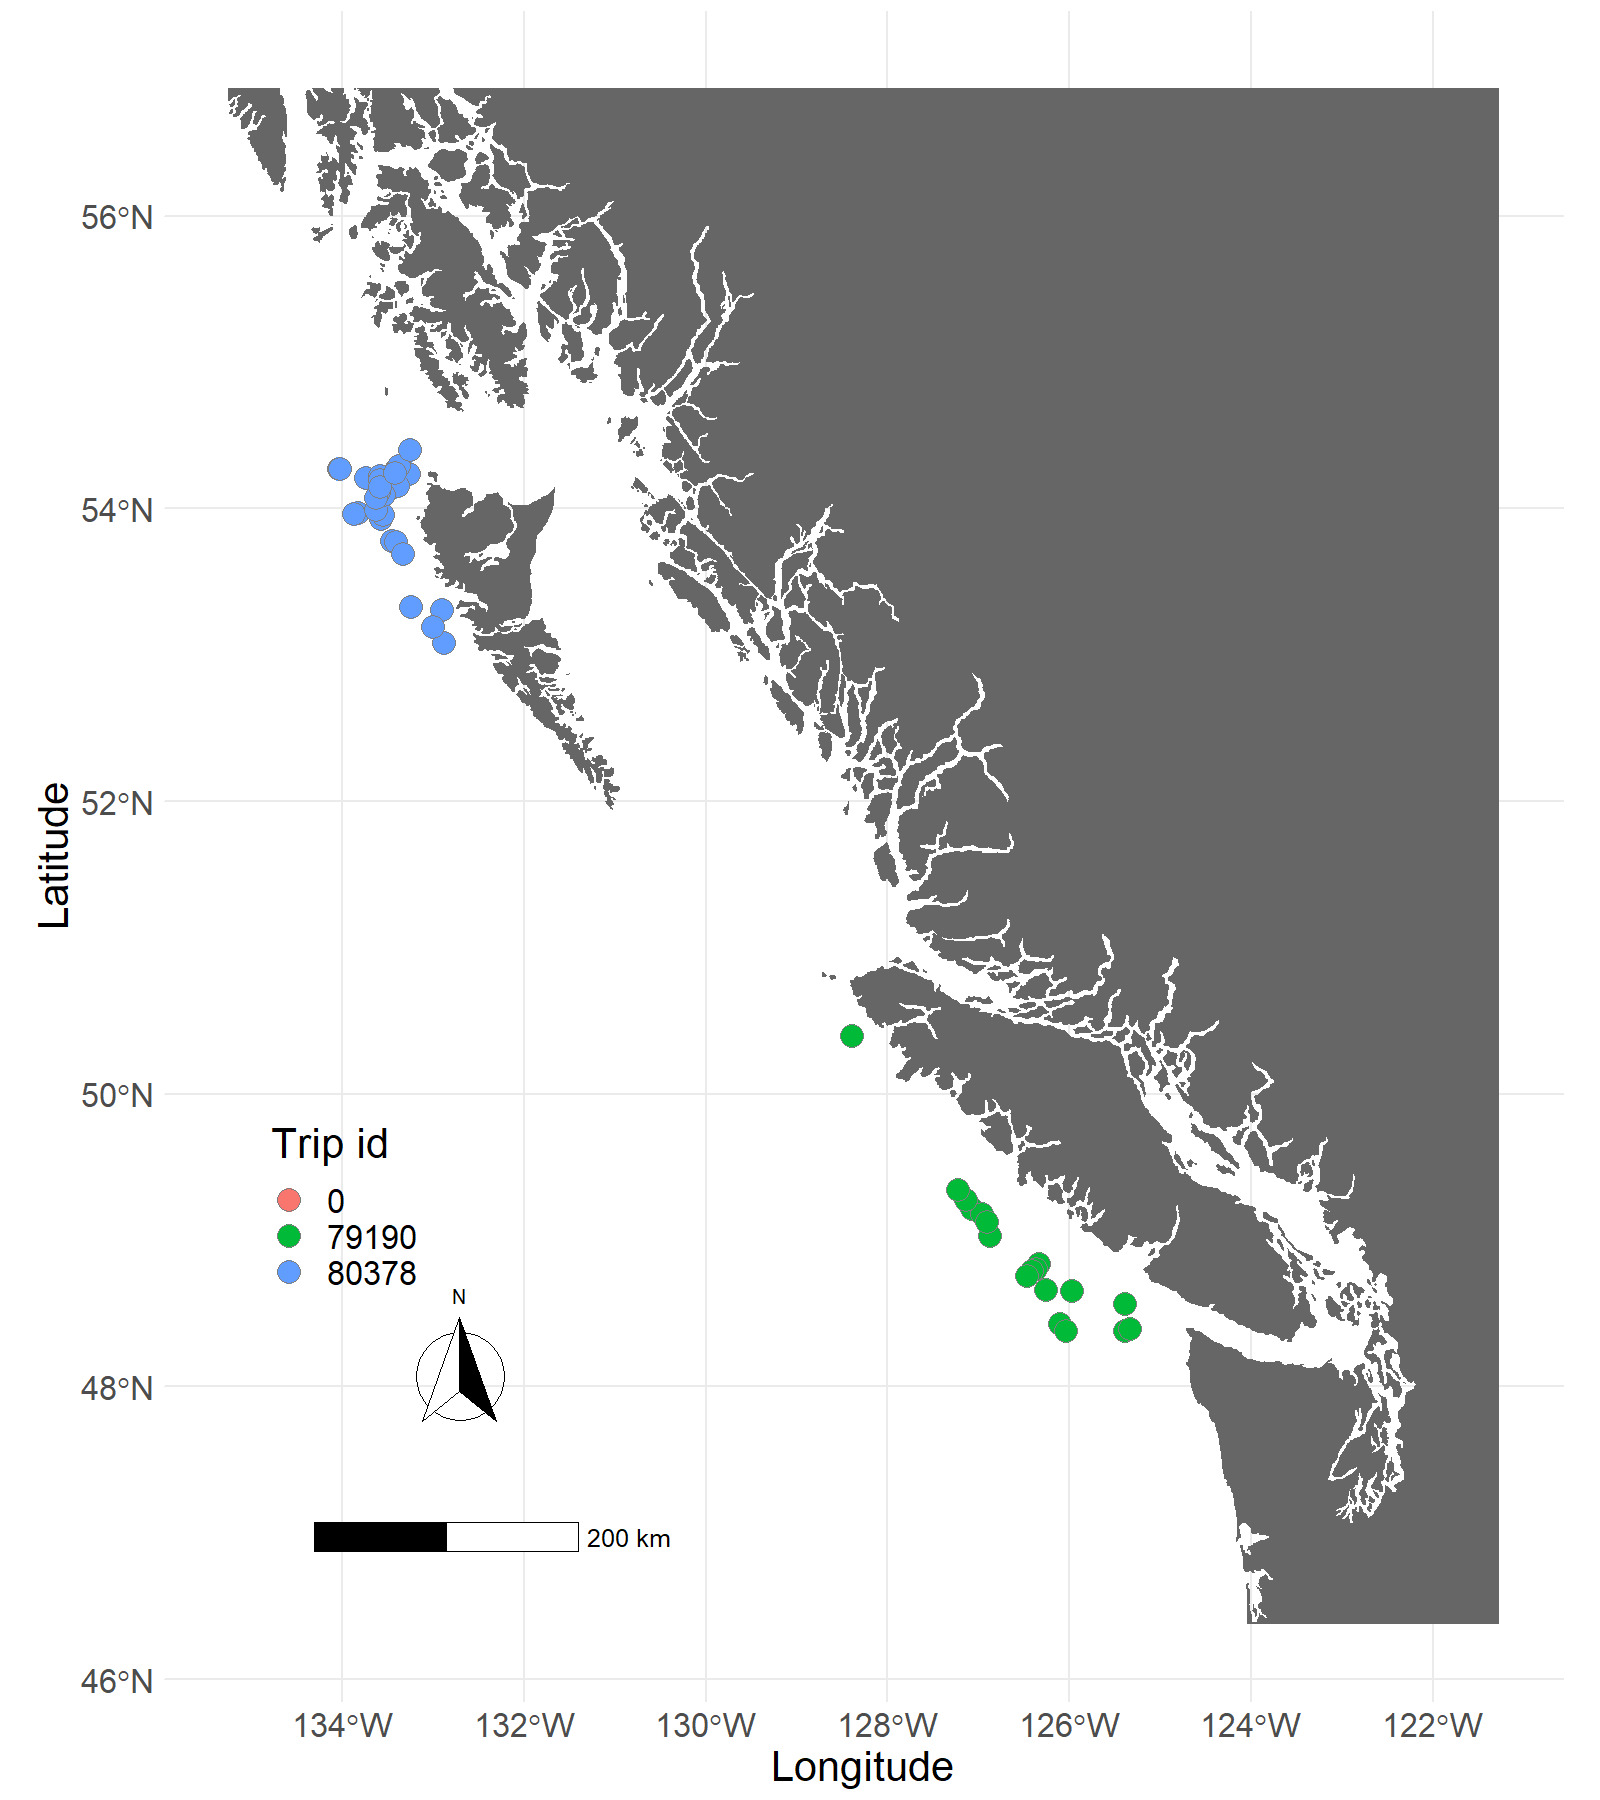
\includegraphics[width=6in]{C:/github/sablehead/figures/Figure1}}{Figure} 

}

\caption{Sample locations from the 2016 WCVI, WCHG and salmon research surveys and 2017 pilot study.}\label{fig:figure1}
\end{figure}

\begin{figure}[htb]

\pdftooltip{\includegraphics[width=470px]{C:/github/sablehead/figures/figure2}}{Figure} \hfill{}

\caption{Relationship between cranial lengths (UJ, ED, ID) vs fork length in millimeters. Predicted points represented by black circles, measured values colored by residual scale.}\label{fig:figure2}
\end{figure}

\begin{figure}[htb]

\pdftooltip{\includegraphics[width=470px]{C:/github/sablehead/figures/figure3}}{Figure} \hfill{}

\caption{Relationship between cranial lengths (SL, PP, PO) vs fork length in millimeters. Predicted points represented by black circles, measured values colored by residual scale.}\label{fig:figure3}
\end{figure}
\clearpage

\begin{appendices}
\counterwithin{figure}{section}
\counterwithin{table}{section}
\counterwithin{equation}{section}

\clearpage

\section{IMAGES OF THE SIX CRANIAL DIMENSION MEASUREMENTS.}
\label{app:first-appendix}

A. Upper jaw measurement (UJ); B. Eye diameter measurement (ED); C. Interorbital distance (ID); D. Snout length (SL); E. Post orbital to preoperculum length measurement (PP); F. Post orbital head length (PO).
\begin{center}\pdftooltip{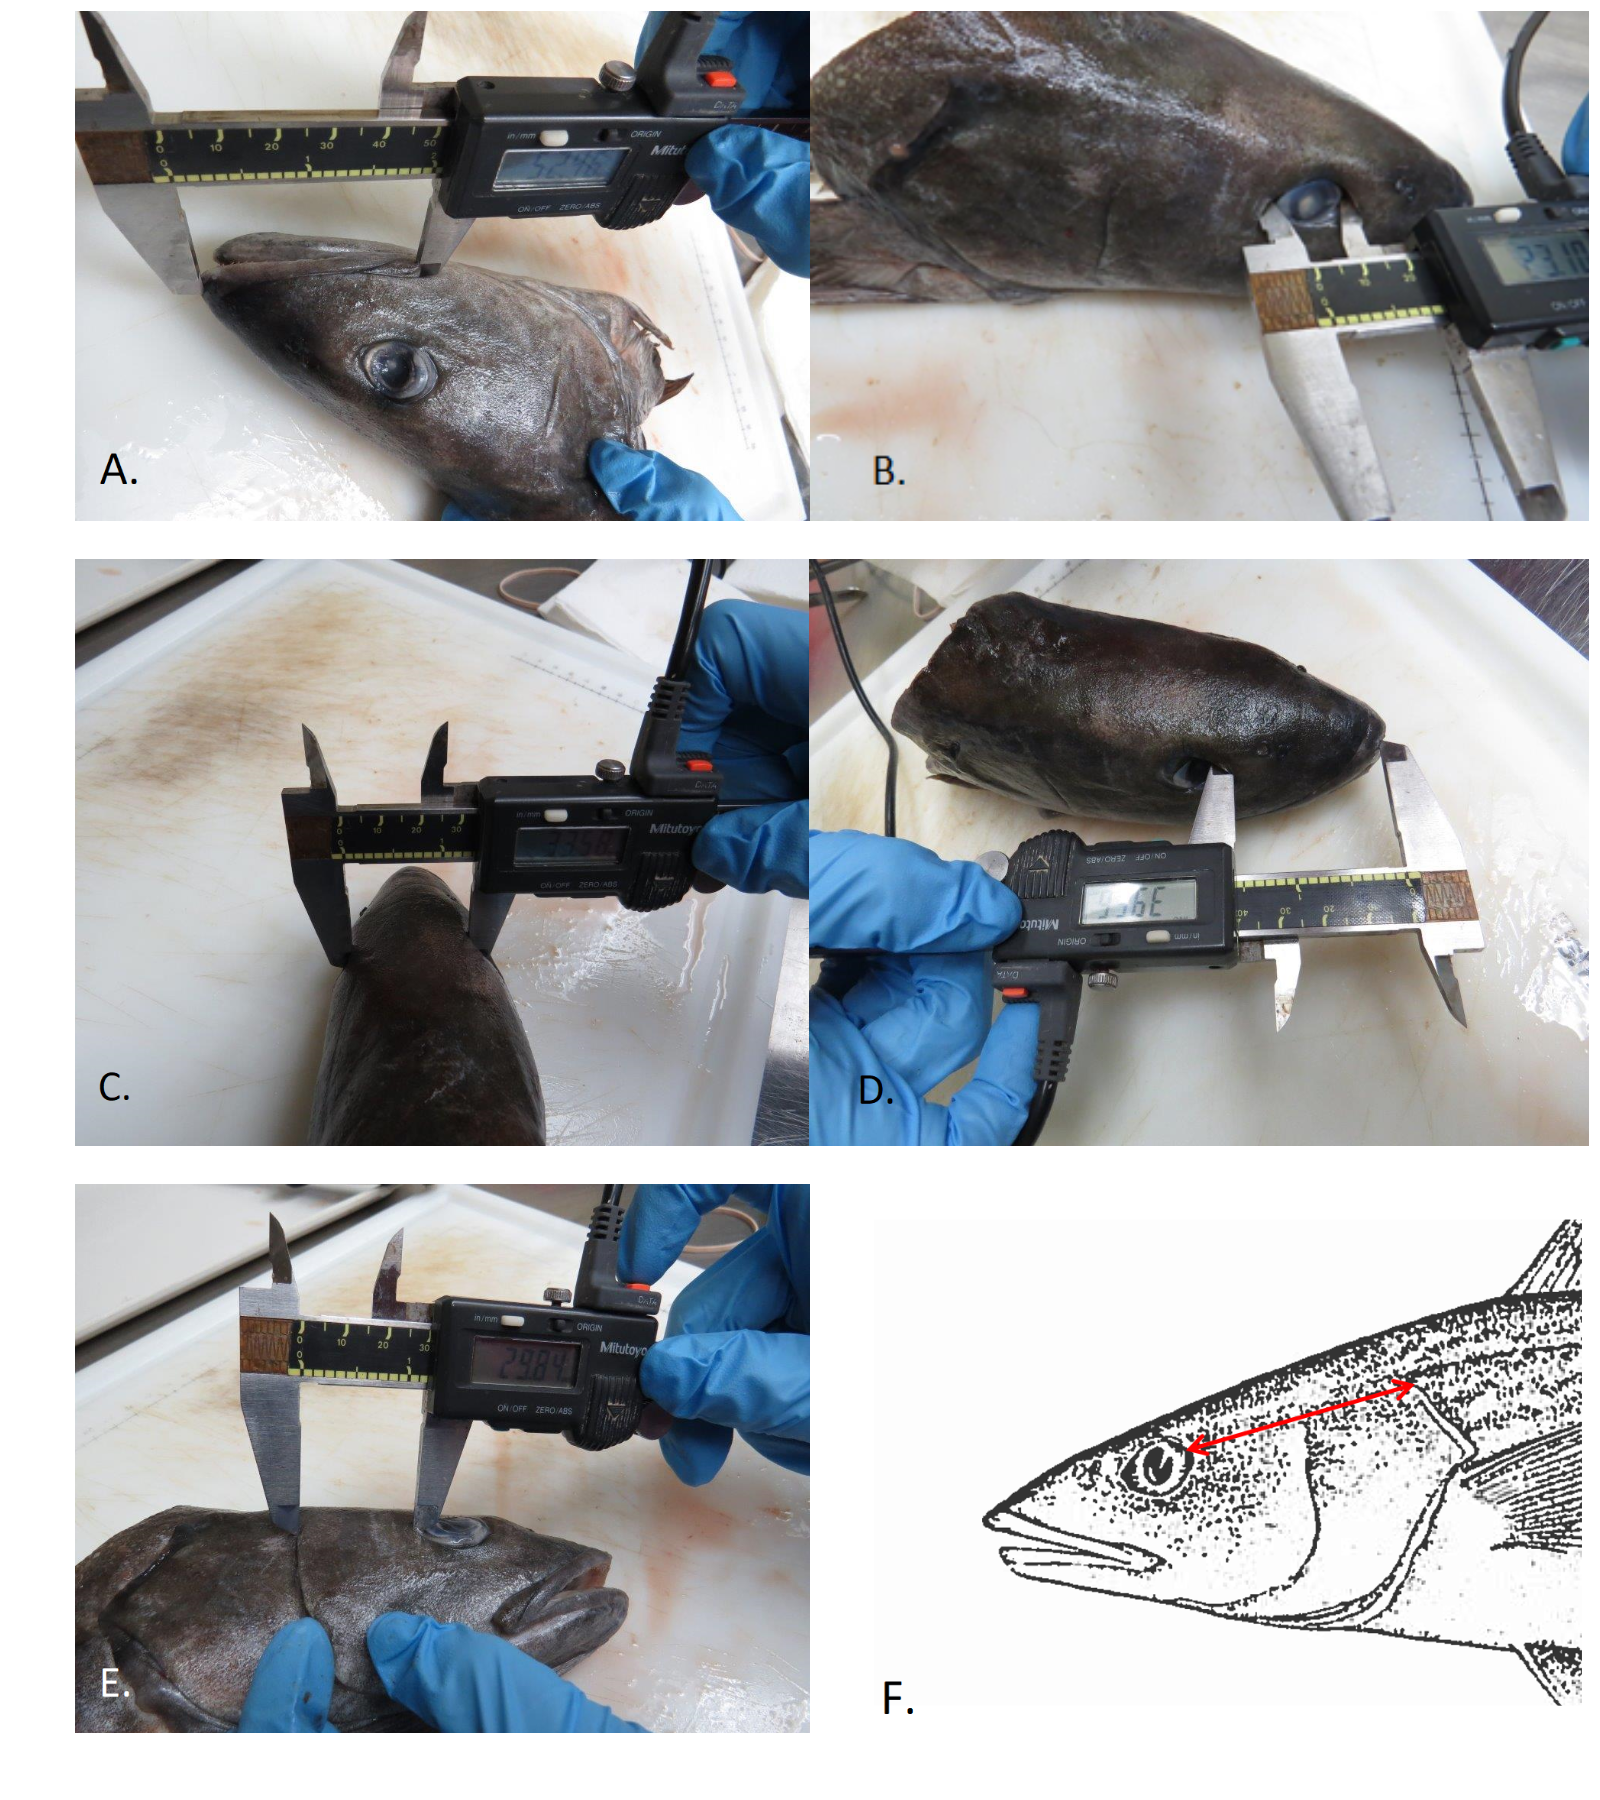
\includegraphics[width=6in]{c:/github/sablehead/figures/AppendixA}}{Figure} \end{center}

\clearpage

\section{SEX DETERMINATION BY OPERCULUM MARKING}
\label{app:second-appendix}

Instructions for sex determinations and operculum knife cuts for sablefish males and females.
\begin{center}\pdftooltip{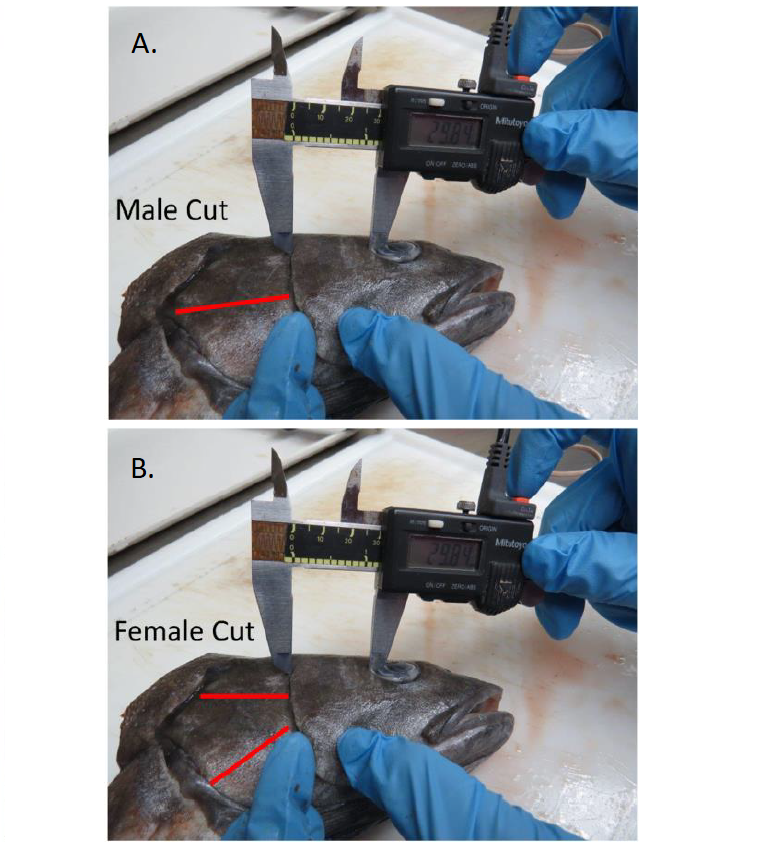
\includegraphics[width=6in]{c:/github/sablehead/figures/AppendixB}}{Figure} \end{center}
\clearpage

\end{appendices}

\clearpage

\hypertarget{references}{%
\section{References}\label{references}}

\noindent \vspace{-2em} \setlength{\parindent}{-0.2in} \setlength{\leftskip}{0.2in} \setlength{\parskip}{8pt}

\hypertarget{refs}{}
\begin{CSLReferences}{1}{0}
\leavevmode{\hypertarget{ref-Cox2019}{}}%
Cox, S.P., Holt, K., and Johnson, S. 2019. Evaluating the robustness of management procedures for the {Sablefish} (*anoplopoma fimbria*) fishery in {British Columbia, Canada} for 2017-18. DFO Can. Sci. Advis. Sec. Res. Doc. 2019/032. vi + 79 p.

\leavevmode{\hypertarget{ref-Haist2001}{}}%
Haist, R.H., V., and Wyeth, M. 2001. Sablefish {Stock Assessment} for 2001 and {Advice to Managers} for 2002. DFO Can. Sci. Advis. Sec. Res. Doc. 2001/135.

\leavevmode{\hypertarget{ref-Isermann2005}{}}%
Isermann, D.A., and Vandergoot, C.S. 2005. Predicting walleye total length from head and mandible measurements. North American Journal of Fisheries Management 25(1): 316--321. Taylor \& Francis.

\leavevmode{\hypertarget{ref-Nottingham2018}{}}%
Nottingham, M.K., Williams, D.C., Wyeth, M.R., and Olsen, N. 2018. Summary of the west coast haida gwaii synoptic bottom trawl survey, august 25 - september 26, 2016. Can. Manuscr. Rep. Fish. Aquat. Sci. 3151: viii: 51 p.

\leavevmode{\hypertarget{ref-Park2007}{}}%
Park, I.S., Kim, Y.J., Choi, H.J., Oh, S.Y., Noh, C.H., and Lee, S.H. 2007. Total length estimation from head dimensions of artificially propagated brown croaker miichthys miiuy. Korean J. Ichthyol. 19: 128--131.

\leavevmode{\hypertarget{ref-Richardson2015}{}}%
Richardson, J., Shears, N., and Taylor, R. 2015. Using relative eye size to estimate the length of fish from a single camera image. Marine Ecology Progress Series 538.

\leavevmode{\hypertarget{ref-Rondeau2013}{}}%
Rondeau, E.B., Messmer, A.M., Sanderson, D.S., Jantzen, S.G., Schalburg, K.R. von, Minkley, D.R., Leong, J.S., Macdonald, G.M., Davidsen, A.E., Parker, W.A., Mazzola, R.S.A., Campbell, B., and Koop, B.F. 2013. Genomics of sablefish (anoplopoma fimbria): Expressed genes, mitochondrial phylogeny, linkage map and identification of a putative sex gene. BMC Genomics 14(1): 452. Journal Article.

\leavevmode{\hypertarget{ref-Serafy1996}{}}%
Serafy, J.E., Schmitz, C.M., Capo, T.R., Clarke, M.E., and Ault, J.S. 1996. Total length estimation of red drum from head dimensions. The Progressive Fish-Culturist 58(4): 289--290. Taylor \& Francis.

\leavevmode{\hypertarget{ref-Shaw1997}{}}%
Shaw, W., and McFarlane, G. 1997. Development of sablefish, anoplopoma fimbira larvae off the west coast of british columbia and transformation in the juvenile stage. NOAA Tech. Rep. NMFS 130: 3--12.

\leavevmode{\hypertarget{ref-Williams2018}{}}%
Williams, D.C., Nottingham, M.K., Olsen, N., and Wyeth, M.R. 2018. Summary of the west coast vancouver island synoptic bottom trawl survey, may 24 - june 15, 2016. Can. Manuscr. Rep. Fish. Aquat. Sci. 3137: viii: 54 p.

\end{CSLReferences}
\end{document}
